% Draft for a 6-page workshop paper (EuroMLSys-style: ACM sigplan, 10pt, two columns).
% Build: latexmk -pdf main.tex   (figures: python paper/figures/make_figures.py)
% Numbers come from results/ via the analysis scripts named in the comments.
% Local build only: this machine lacks Libertine; Overleaf uses the real ACM fonts.
\PassOptionsToPackage{expansion=false}{microtype}
\documentclass[sigplan,10pt]{acmart}
\IfFileExists{libertine.sty}{}{\usepackage{lmodern}}
\settopmatter{printacmref=false, printfolios=true}
\renewcommand\footnotetextcopyrightpermission[1]{}
\setcopyright{none}
\acmConference[Draft]{Workshop draft}{2026}{}
\usepackage{booktabs}
\setlength{\emergencystretch}{2.5em}
\usepackage{multirow}
\newcommand{\pct}[1]{#1\%}
\newcommand{\todo}[1]{\textcolor{red}{[TODO: #1]}}

\begin{document}

\title{Where Does the Time Go When Embodied Agents Share a GPU?}
\subtitle{Scheduling, Co-location, and Batching for Batch Evaluation of a VLA Agent Harness}

\author{Zixin Wan}
\affiliation{\institution{Columbia University}\city{New York}\country{USA}}
% \todo{advisor / co-authors}

\begin{abstract}
Evaluating embodied agents means running many episodes at once: an LLM planner, a
vision-language-action model (VLA), grounding and segmentation models, and a physics
simulator, all sharing one GPU and a CPU quota. We measure where the time goes in
such batches with RPent, an agent harness that drives Pi0.5, Molmo2 and SAM3 on
LIBERO-PRO, and test three levers on an A100. (1) Episode launch order shortens a
batch by \pct{6}--\pct{13}; a per-task history of past runtimes is a better length
estimate than the agent's own plan (Spearman 0.97 vs.\ 0.58 on held-out tasks).
(2) Co-locating a local 7B VLM planner with the robot models slows every model by
1.3--3.3$\times$ under default GPU time-slicing; enabling MPS removes most of it and
shortens agent-like batches by \pct{24}--\pct{30}, while pausing the planner during VLA
bursts gives nothing on top of MPS. (3) Batching VLA calls across episodes cuts
makespan by \pct{36}--\pct{51} when the VLA dominates an episode but by nothing on real
plan-replay episodes, where the VLA is only \pct{11}--\pct{12} of the time and the
simulator and client-side Python take over half. Plan-level ``intent'' carried
information in every experiment but never beat a simple baseline. We report these
results, including the negative ones, with the measurement pitfalls we hit.
\end{abstract}

\maketitle

% ---------------------------------------------------------------------------
\section{Introduction}

Embodied agents are increasingly built as harnesses: a planner (an LLM or a stored
plan) calls a frozen VLA policy, perception models, and scripted motion primitives as
tools inside a simulator~\cite{rpent,pi05}. Evaluating one checkpoint, prompt or planner
means hundreds of such episodes, and the cheapest way to run them is to pack many
onto one GPU that serves all models. Whoever runs those batches has to decide how to
order the episodes, how the models share the GPU, and whether to batch model calls.

Systems work on robot-model serving has focused on request-level scheduling and
batching from runtime history~\cite{kairos,armory,rosa}, and evaluation harnesses have
scaled VLA rollouts by sharding and batching synchronous environments~\cite{vlaeval}.
A natural further idea, and the starting point of this project, is to use the plan
itself: a tool call such as \texttt{pi0\_pick(max\_chunks=12)} announces the coming
VLA work before it happens. We tested that idea three times and report what we found
instead: where the time actually goes, which generic mechanisms help, and why the
plan's advance notice did not matter.

\paragraph{Findings.}
\begin{itemize}
\item \textbf{The GPU models are a minority of episode time} in plan-replay batches:
  \pct{22} at 8 concurrent episodes, \pct{35} at 16, against \pct{32}--\pct{36} in the
  simulator and \pct{24}--\pct{32} in client-side Python (\S\ref{sec:breakdown}).
\item \textbf{Episode-level launch ordering} (JIT-LPT) shortens a batch by
  \pct{13.1} on one task set and \pct{5.8} on held-out tasks; request-level reordering
  has at most \pct{2} of headroom before saturation. Per-task history estimates beat
  plan-derived ones (\S\ref{sec:launch}).
\item \textbf{Co-locating a local planner} on the robot GPU slows the VLA 2.2$\times$
  regardless of planner load because processes take turns on the GPU; MPS turns
  this into 1.1--1.5$\times$ and shortens batches by up to \pct{30}; pausing the
  planner during VLA bursts does not help on top of MPS (\S\ref{sec:coloc}).
\item \textbf{Batching VLA calls} helps exactly in proportion to the VLA's share of
  the episode: \pct{36}--\pct{51} on a VLA-heavy synthetic workload, nothing on real
  episodes (\S\ref{sec:batch}).
\end{itemize}
We close with the measurement pitfalls that, uncorrected, would have changed several
of these conclusions (\S\ref{sec:lessons}).

% ---------------------------------------------------------------------------
\section{System and Methodology}\label{sec:setup}

\paragraph{Workload.} RPent~\cite{rpent} runs LIBERO-PRO~\cite{liberopro} manipulation
tasks. Each episode is a process that talks to an environment server (MuJoCo) and to
shared model servers over HTTP: Pi0.5~\cite{pi05} for VLA action chunks, Molmo2-8B for
pointing/grounding~\cite{molmo}, and SAM3 for segmentation~\cite{sam3}. We use RPent's
Flash mode, which replays a plan written once by a frontier LLM (78 plans over 8
suites): the plan fixes the sequence of primitives (\texttt{move\_to},
\texttt{pi0\_pick} with a \texttt{max\_chunks} budget, grounding calls), while
perception and the VLA run live. Each server handles one request at a time (RPent's
facades hold an exclusive lock).

\paragraph{Instrumentation.} A drop-in launcher patches RPent at runtime to log every
tool call and RPC and to tag requests with episode and tool-call ids; a proxy in front
of each model server logs queueing and service time and implements ordering and
batching policies. A sweep driver runs $N$ concurrent episodes from a batch, records
cgroup CPU quota and throttling, and pairs arms on identical shuffled batches.

\paragraph{Platform and statistics.} One NVIDIA A100-SXM4-80GB (RunPod), with a
cgroup quota of about 13.6 CPUs. Comparisons are paired by repeat (same episodes,
same initial order), arm order rotates between repeats, the first cell of a session
is a discarded warm-up, and we report means with 95\% $t$-intervals. Cells with CPU
throttling above \pct{5} of makespan are flagged. For scheduling studies beyond what
we ran on the GPU, a trace-driven simulator replays 959 recorded episodes (local time
as recorded, model calls as single-server queues); it matched six real FIFO cells to
within about one second and predicted the GPU launch-order result within one point.

% ---------------------------------------------------------------------------
\section{Where the Time Goes}\label{sec:breakdown}

\begin{figure}[t]
  \centering
  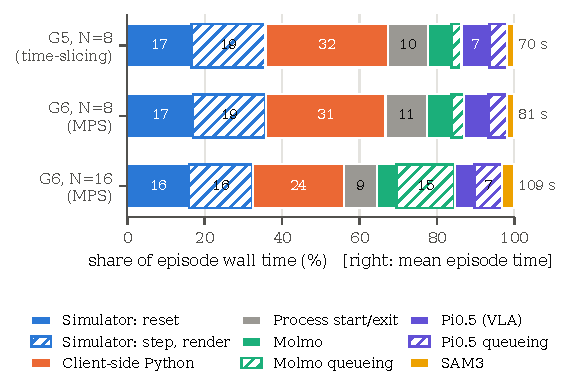
\includegraphics[width=\columnwidth]{figures/breakdown.pdf}
  \caption{Episode wall time by component, summed over all episodes of a configuration
  (G5: 149 episodes; G6: 90 per level). Hatched: time queued at the model's proxy.
  ``Client-side Python'' is time inside the episode between RPCs.}
  \label{fig:breakdown}
\end{figure}

Figure~\ref{fig:breakdown} splits every episode's wall time using the client-side RPC
log and the proxies' queueing times (RPCs within an episode are sequential, so the parts
add up exactly). Three groups dominate:
\begin{itemize}
\item \textbf{The simulator}, \pct{32}--\pct{36}: environment reset alone is
  \pct{16}--\pct{17} (12--18\,s per episode), stepping and rendering another
  \pct{16}--\pct{19}.
\item \textbf{Client-side Python}, \pct{24}--\pct{32}: scripted motion, plan replay,
  and encoding observations for RPCs. Process start and exit add \pct{9}--\pct{11}.
\item \textbf{The GPU models}, \pct{22} at $N=8$ and \pct{35} at $N=16$. An episode
  makes only about 18--20 VLA calls and 3.3 Molmo calls. Growth with $N$ is mostly
  queueing at Molmo, which rises from \pct{3} to \pct{15} of episode time.
\end{itemize}
Earlier sweeps show the same order of contention: going from $N=8$ to $N=16$,
episodes/hour \emph{dropped} from 225 to 194 on this CPU quota, Molmo waiting rose
from \pct{5.8} to \pct{22.8} of episode time (median call: 1.1\,s at $N=1$, 11.2\,s at
$N=16$),
and the VLA was busy only \pct{25}--\pct{32} of the time. In simulation with enough
CPU, throughput saturates near $N=24$ at $\approx$375 episodes/hour, when Molmo
reaches \pct{81} utilization and the VLA \pct{76}.

\textbf{Takeaway:} for plan-replay agents, the shared GPU models are not the main
cost; the simulator, the client, and serialized Molmo calls are. Mechanisms that only
speed up VLA serving have a ceiling of roughly a tenth of episode time.

% ---------------------------------------------------------------------------
\section{Episode-level Launch Ordering}\label{sec:launch}

\paragraph{Request-level reordering has little headroom.} Replaying 128-episode
batches in the simulator, reordering the Molmo and VLA queues by remaining work
(SRPT) improves mean episode time by at most \pct{2} up to $N=16$, even with oracle
knowledge; the gains appear only past saturation ($N\geq32$: \pct{7}--\pct{21} for the
oracle). Our real GPU runs at $N=8$ and 16 showed no significant effect, consistent
with that bound.

\paragraph{Launch order does have headroom.} A batch's makespan is often set by a few
long episodes launched late. Classic LPT~\cite{graham} (longest first) helps small
batches but \emph{slows} 128-episode batches by \pct{5}: it starts all long episodes
together and they contend for Molmo. JIT-LPT launches the longest pending episode
only when, at the current completion rate, it would otherwise become the tail, and
the next one in the given order otherwise. In simulation it never loses to random
order (\pct{4}--\pct{18} shorter makespan) and is insensitive to its one knob.

\begin{table}[t]
  \centering\small
  \caption{GPU makespan change from JIT-LPT vs.\ random launch order ($N=8$, 32
  episodes, FIFO queues, paired repeats).}
  \label{tab:launch}
  \resizebox{\columnwidth}{!}{%
  \begin{tabular}{@{}lccc@{}}
  \toprule
  Tasks, estimate & change & 95\% CI & faster \\
  \midrule
  G4: tuning tasks, plan & \textbf{\pct{-13.1}} & $[-20.6, -5.6]$ & 8/8 \\
  G5: held-out, history & \textbf{\pct{-5.8}} & $[-10.3, -1.3]$ & 5/5 \\
  G5: held-out, plan & \pct{-3.0} & $[-6.9, +1.0]$ & 4/5 \\
  G5: held-out, history, half cold & \pct{-1.2} & $[-6.7, +4.2]$ & 3/5 \\
  \midrule
  G5: oracle (simulated) & \pct{-9.9} & $\pm1.5$ & -- \\
  \bottomrule
  \end{tabular}}
\end{table}

\paragraph{GPU results and the source of the estimate.} Table~\ref{tab:launch} shows
the GPU runs. On the 16 tasks used to build the cost table that turns a plan into
seconds (G4), plan-based JIT-LPT cut makespan by \pct{13.1} and made it more
predictable (375--422\,s vs.\ 425--504\,s). On 16 held-out tasks drawn at random
(G5), a per-task history of mean runtimes from one earlier run was the best estimate
(\pct{-5.8}); the plan estimate was not significant, and with half the tasks unseen
the history lost most of its benefit. The plan's rank correlation with actual
duration fell from 0.87 on the tuning tasks to 0.58 on held-out tasks (history:
0.97), and refitting the cost model by leave-one-suite-out did not recover it (0.67).
The plan is an upper bound: \texttt{max\_chunks} is a budget that picks usually end
early, and it cannot foresee retries. The batch was also more homogeneous
(coefficient of variation 0.44), so even the oracle gains only \pct{9.9}.

\textbf{Takeaway:} order episodes, not requests; estimate lengths from history when
the tasks have run before, and treat plans as a cold-start fallback.

% ---------------------------------------------------------------------------
\section{Co-locating a Local Planner}\label{sec:coloc}

In an agentic setting the planner is itself a GPU model. We served Qwen2.5-VL-7B
with vLLM~\cite{vllm,qwen25vl} on the same A100 (\pct{32} of memory) beside Pi0.5,
Molmo2 and SAM3, and measured each model under closed-loop synthetic load (planner:
streamed completions with an image and a $\approx$3.5k-token prompt, 256 output
tokens; VLA: back-to-back predicts with the 0.17\,s environment step between them).

\begin{figure}[t]
  \centering
  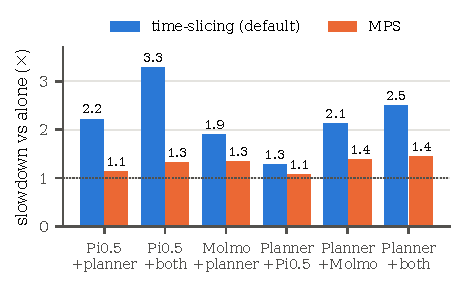
\includegraphics[width=\columnwidth]{figures/colocation.pdf}
  \caption{Slowdown of each model when co-located, relative to running alone (median
  latency; planner: time per output token), under default time-slicing and under MPS.
  Planner: 4 streams.}
  \label{fig:coloc}
\end{figure}

\paragraph{Time-slicing, not saturation.} Under the default setting, Pi0.5 is
2.2$\times$ slower whenever the planner decodes, and the slowdown is the same with 1,
4 or 16 planner streams (2.29, 2.22, 2.28$\times$). The cause is not compute
saturation but the GPU alternating between processes: the decode loop always has
kernels queued, so each VLA call waits for its turns. Molmo, itself autoregressive,
and the planner slow each other by about 2$\times$; with all three, the VLA is
3.3$\times$ slower (Fig.~\ref{fig:coloc}).

\paragraph{MPS removes most of it.} With NVIDIA MPS, which lets kernels from
different processes run concurrently, the same pairs slow down by only 1.1--1.5$\times$.
The price is about \pct{25} on a model running alone (Pi0.5: 0.165$\rightarrow$0.204\,s).
On agent-like batches (each episode alternates a planner call, an optional Molmo call
and a burst of 4--16 VLA chunks), MPS alone shortens makespan by \pct{30.1}
($\pm2.7$, $N=8$) and \pct{24.2} ($\pm11.7$, $N=4$).

\begin{table}[t]
  \centering\small
  \caption{Pausing the planner (SIGSTOP) during VLA bursts, $N=8$ agent-like batches,
  makespan change vs.\ no coordination on the same GPU setup. ``Paused'': fraction of
  the batch with the planner frozen.}
  \label{tab:pause}
  \resizebox{\columnwidth}{!}{%
  \begin{tabular}{@{}llrr@{}}
  \toprule
  Setup & Policy (budget) & change & paused \\
  \midrule
  \multirow{3}{*}{time-slicing} & always during bursts & \pct{-3.6} $\pm9.0$ & \pct{72} \\
   & by announced length (2\,s) & \pct{-14.0} $\pm4.3$ & \pct{47} \\
   & by true length (2\,s) & \pct{-11.5} $\pm0.9$ & \pct{63} \\
  \midrule
  \multirow{4}{*}{MPS} & by announced length (1\,s) & \pct{-2.8} $\pm5.1$ & \pct{15} \\
   & by announced length (4\,s) & \pct{+15.6} $\pm6.6$ & \pct{71} \\
   & by true length (4\,s) & \pct{+25.7} $\pm14.3$ & \pct{74} \\
   & static: planner at \pct{30} of SMs & \pct{-5.8} $\pm7.2$ & -- \\
  \bottomrule
  \end{tabular}}
\end{table}

\paragraph{Pausing the planner does not help on top of MPS} Tool calls announce VLA
bursts, so a coordinator can freeze the planner server while a burst runs (we used
SIGSTOP/SIGCONT on the vLLM process tree as an upper-bound prototype, with an
anti-starvation guard). Without MPS, pausing only near the end of a burst helps
(\pct{-14}); unconditional pausing brings the VLA back to its solo latency (0.21\,s) but
inflates planner calls from 2.6 to 11\,s and makes the batch slower. Under MPS, no
policy is significantly better than doing nothing, and every policy gets worse as it
pauses more (Table~\ref{tab:pause}). Policies using the announced \texttt{max\_chunks}
do best in every row, but because the budget overstates the burst and so pauses
less, not because the information is better: the true length does worse. Co-located
work overlaps usefully (sharing the GPU, Pi0.5 keeps \pct{63} of its solo throughput
and the planner \pct{80}, more than strict alternation would allow), and pausing gives
that overlap away.

\textbf{Takeaway:} turn on MPS before anything else; it is a configuration change
worth \pct{24}--\pct{30} here, and the obvious intent-driven refinement adds nothing.

% ---------------------------------------------------------------------------
\section{Batching VLA Calls}\label{sec:batch}

\begin{figure}[t]
  \centering
  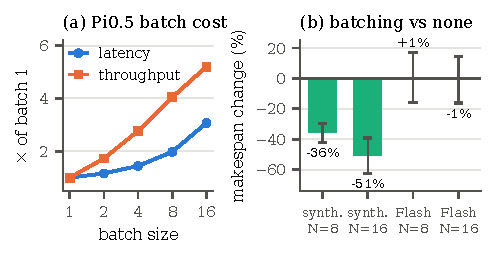
\includegraphics[width=\columnwidth]{figures/batching.pdf}
  \caption{(a) Pi0.5 latency and throughput vs.\ batch size, relative to batch 1 (MPS,
  4 planner streams). (b) Makespan change from greedy cross-episode batching vs.\ none,
  on the agent-like synthetic workload and on real RPent Flash episodes (MPS; error
  bars: 95\% CI).}
  \label{fig:batch}
\end{figure}

RPent's Pi0.5 server accepts batched observations, but every agent sends one at a
time. A batch of 8 costs only 1.93--1.98$\times$ a batch of 1, so throughput grows
4$\times$ (5.2$\times$ at 16; Fig.~\ref{fig:batch}a). We added a batching policy to
the proxy that merges waiting \texttt{vla.predict} calls into one call and splits the
actions back by row, with three dispatch rules: \emph{greedy} (send everything waiting
when the server frees up), a fixed \emph{window} of 10 or 30\,ms, and \emph{predictive}
waiting (hold a batch while another episode inside a pick is expected to send its next
chunk; optionally using the pick's remaining \texttt{max\_chunks} to stop waiting for
episodes whose pick is over).

On the agent-like workload of \S\ref{sec:coloc}, greedy batching shortens makespan by
\pct{35.8} ($N=8$) and \pct{50.8} ($N=16$); every waiting rule lands within about three points of
it (\pct{-38} to \pct{-39} and \pct{-52} to \pct{-53}), and the predictive rule chose to
wait in only about \pct{3} of batches. On real Flash episodes (the G5 held-out batch,
3 repeats), neither greedy nor intent-aware batching changed makespan significantly
(Fig.~\ref{fig:batch}b, intervals $\pm$13--21 points): batches averaged only 1.2--1.7
requests and the median VLA queueing was 0.1--0.2\,s. This is exactly what
\S\ref{sec:breakdown} predicts: the synthetic workload issues 3--6 bursts of 4--16
chunks with no simulator time, while a real episode makes about 18 VLA calls in
80--110\,s.

\textbf{Takeaway:} batching is worth up to half the makespan when the VLA dominates
episode time (as in policy-only rollouts~\cite{vlaeval}) and nothing when it does not;
check the VLA's share before building it, and calibrate synthetic workloads on real
traces.

% ---------------------------------------------------------------------------
\section{Lessons and Pitfalls}\label{sec:lessons}

\paragraph{Intent was informative but never decisive.} The plan predicts per-primitive
VLA calls far better than the last round's count (mean error 2.7 vs.\ 9.0 calls,
leave-one-task-out), and remaining work better than history mid-episode (Spearman
0.76 vs.\ 0.02). Yet in each mechanism a simpler signal or a generic mechanism won:
history for launch order, MPS for co-location, greedy dispatch for batching. When
episodes are repetitive, history is cheap and accurate; when resources overlap,
utilization matters more than foresight.

\paragraph{Pitfalls that changed conclusions.}
\begin{itemize}
\item \emph{Thread oversubscription.} Containers report the host's 128 cores to
  OpenMP/BLAS while the quota is 13.6; unbounded thread pools made
  \texttt{env.step} 60$\times$ slower (2.3\,s vs.\ 38\,ms) and turned a GPU study into a
  CPU one. Pin threads per process and log cgroup throttling.
\item \emph{Cold start.} In the first cell of a session, episodes took 25.7\,s instead
  of about 20\,s to start, which produced an apparent \pct{7} scheduling gain;
  discard a warm-up cell.
\item \emph{Selection bias in estimator quality.} Plan correlation was 0.82--0.87 on
  the tasks chosen for their varied plans and 0.58 on random ones.
\item \emph{Closed-loop synchronization.} Closed-loop planner streams synchronize, so
  time-to-first-token looked 2$\times$ \emph{better} under interference.
\item \emph{Silent load generators.} A planner that was down turned a ``with planner''
  measurement into a solo one; check that background load actually completes requests.
\item \emph{Synthetic workloads.} Uncalibrated burst sizes overstated the VLA's share
  and the value of batching by an order of magnitude.
\item \emph{Broken tasks.} 3 of 78 Flash tasks never start in LIBERO-PRO; arms must
  share them to stay paired.
\end{itemize}

% ---------------------------------------------------------------------------
\section{Related Work}

\emph{Robot-model serving.} Kairos~\cite{kairos} prioritizes VLA requests by wait ratio
with last-round runtimes; ROSA~\cite{rosa} places robot foundation models on a shared
pool with admission and rate limits; Armory~\cite{armory} batches $\pi_{0.5}$ chunks
across robots; Robion~\cite{robion} partitions SMs between VLM and action stages. All
schedule requests or chunks from runtime state; we study episode launch order,
co-location with a planner, and when batching pays off in an agent harness.
\emph{Evaluation at scale.} vla-eval~\cite{vlaeval} speeds up VLA evaluation by
sharding environments and batching their synchronous steps; our episodes are
asynchronous, and the simulator dominates them too. EnvPool~\cite{envpool} batches
environment execution for RL. \emph{Length-aware LLM serving} predicts output lengths
to approximate SJF~\cite{fu2024ltr}; we compare plan-derived and history-derived
episode lengths. \emph{GPU sharing.} MPS and MIG are the standard mechanisms; recent
LLM-agent servers partition SMs dynamically~\cite{agentserve}. \emph{Agent
characterization.} Wan et~al.~\cite{wan2025ispass} find planning and communication
dominate LLM-driven embodied agents; we characterize the plan-replay regime, where the
simulator and client dominate.

% ---------------------------------------------------------------------------
\section{Limitations and Conclusion}

All GPU results use one A100, one harness, plans from one planner, and batches of
12--48 episodes at $N\leq16$; larger-scale scheduling claims come from a simulator
that overestimated held-out gains by 2--4 points. The co-location and batching studies
use a synthetic agent workload for the planner side, SIGSTOP is an upper-bound
mechanism, and several cells have only three repeats. The G6 cells ran under
\pct{5}--\pct{10} CPU throttling. \todo{rerun G6 on a pod with a larger CPU quota, or
report it as is.}

For batch evaluation of embodied agents on one GPU, the levers that mattered were
configuration and ordering: enable MPS, launch long episodes early using history, and
batch the VLA only if it is a large share of episode time. In this setting, the most
useful use of the agent's plan was as a fallback when no history exists.

\bibliographystyle{ACM-Reference-Format}
\bibliography{refs}

\end{document}
